\chapter{Background}
\label{ch:background}

This chapter provides the background knowledge relevant for the thesis work. It
will initially discuss graph and related problems (\autoref{sec:signed_graphs_and_density}) which are significant in the
following used methodologies, as well as concepts of computational complexity
(\autoref{sec:computational_complexity_and_approximability}) and \acrlong{LP} (\autoref{sec:linear_and_mixed_integer_programming}).

\section{Signed graphs and density}%
\label{sec:signed_graphs_and_density}

A \emph{graph} is a collection of \emph{vertices} or \emph{nodes} $V$ and
\emph{edges} or \emph{links} $E$ between the nodes, representing relationships
between entities; this structure turns out to be very useful in
representing many interesting concepts from social sciences, biology, physics,
chemistry and geography (\autoref{fig:tex/img/sample-graph})\cite{Newman2018}\cite{Menczer2020}.

\begin{figure}
	\centering
	\includegraphics[width=0.6\linewidth]{tex/img/sample-graph.png}
	\caption{The retweet network of posts regarding US during 2010 midterm
		elections. Red and blue nodes are associated with conservative and
		progressive users, respectively \cite{Menczer2020}}%
	\label{fig:tex/img/sample-graph}
\end{figure}

\paragraph{Different types of graphs}%
\label{par:different_types_of_graphs}

In its simplest form graph are \emph{undirected} and \emph{unweighted}. In an
\emph{undirected} graph relationships are bi-directional, while in directed graph
the order of nodes in a link reflects the
direction (i.e. an edge $e_{ij} $ is different from an edge $e_{ji} $). A weighted
graph instead associates a weight $\omega $ to each edge
\cite{Menczer2020}\cite{AlbertLaszloNortheasternUniversity2016}.

Sometimes also edges are allowed to be either positive or negative (for example when
definying the relationships in a acquaintance network): these king of networks
are usually called \emph{signed graphs} \cite{Newman2018}.

\subsection{Densest subgraphs}%
\label{sub:densest_subgraphs}

Finding dense subgraphs is a problem which has received a lot of attention and
has been studied a lot, and different definitions have been adopted
\cite{charikar2000greedy}\cite{asahiro1995finding}\cite{asahiro2000greedily}
\cite{feige1997densest}.

We will refer to the definition in \cite{charikar2000greedy} and presents some
of its results which are used and important for the development of the methods
in the following chapters.



\clearpage

\section{Computational complexity and \\approximability}%
\label{sec:computational_complexity_and_approximability}

Complexity Theory deals with the study of the intrinsic complexity of
computational tasks; more specifically it mainly aims at determining the
complexity of any given task. It also elaborates on the relationships between
the complexity of different problems, for example proving that 2 problems are
computationally equivalent\cite{9780521884730}, through a notion called
\emph{reduction}.

\subsection{Complexity classes}%
\label{par:complexity_classes}

According to their complexity, problems can be divided in different groups
\cite{DemaineFall2014}.

\paragraph{$\mathcal{P} $}%
\label{par:p}
is the set of problems which can be solved in polynomial time in the size $n$ of
the problem, i.e. $n^{O(1)} $. In this set there are problems such as Linear
Programming Models \cite{KHACHIYAN198053}\cite{Karmarkar1984}, finding whether
or not a graph is connected \cite{9780521884730}.

\paragraph{$\mathcal{NP} $}%
\label{par:np} is the set of problems whose solution can be verified in
polynomial time in the size $n$ of the problem, i.e. $n^{O(1)} $.

According to these definition it is easy to see that $\mathcal{P} \subseteq
	\mathcal{NP} $. A common $\mathcal{NP} $ problem is factoring, i.e. finding a
prime factor $p$ of a number $N$ in a given interval \cite{SanjeevArora2017}.

\paragraph{$\mathcal{NP} $-Hard}%
\label{par:_np_hard} is the set of problems that are \emph{at least as hard} as
any other problem in $\mathcal{NP} $. Some well-known $\mathcal{NP} $-Hard
problems are the $\textsc{Sat}$ (deciding whether a boolean formula can be
satisfied or not) and the $\textsc{MaxClique}$ (finding the biggest complete
subgraph), as shown is a famous paper by Karp \cite{Miller1972} (see
\autoref{fig:tex/img/post_vaccine_social_scheduling} ).

\begin{figure}[]
	\centering
	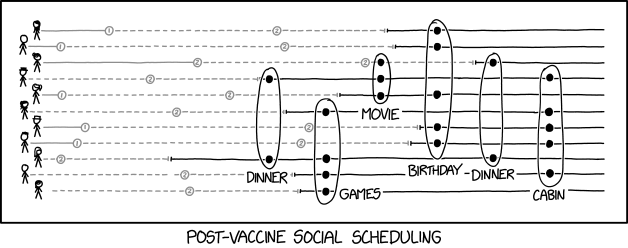
\includegraphics[width=0.8\linewidth]{tex/img/post_vaccine_social_scheduling.png}
	\caption{\emph{As if this problems weren't $\mathcal{NP} $-Hard enough}.
		Post-vaccine social scheduling may be $\mathcal{NP} $-Hard \cite{Munroe}}%
	\label{fig:tex/img/post_vaccine_social_scheduling}
\end{figure}

\paragraph{$\mathcal{NP} $-Complete}%
\label{par:_np_hard} is the set of problems in $\mathcal{NP} $-Hard that are
also in $\mathcal{NP} $. Intuitively these correspond the most difficult
problems to solve in $\mathcal{NP} $. The number of problems which are known to
be in this set is in the order of a thousand \cite{SanjeevArora2017}.

\subsection{$\mathcal{P} $ vs $\mathcal{NP}$}%
\label{sub:_p_vs_np_}

A fundamental question in Computational Complexity is wheter $\mathcal{P} =
	\mathcal{NP} $. Mostly people believe that this is not true, so
$\mathcal{P} \neq \mathcal{NP} $, and also our daily experience tell us that
often it is easier to check the correctness of a solution of a problem than
finding it \cite{9780521884730}: in many cases coming up with the correct
answer requires searching over an exponentially large set
\cite{SanjeevArora2017}. Nonetheless no mathematical proof of this notion has
been found and, in fact, in the last decades there has been little or no progress towards it \cite{Erickson2019}.

If, it is mostly accepted, $\mathcal{P} \neq \mathcal{NP} $ this would produce
a situation as depicted in \autoref{fig:tex/img/complexity-diagram}:
there are problems for which we are not able to find the solution
efficiently (i.e. in polynomial time). On the other side this allows the
existance of one-way-functions (i.e. functions whose inverse is much harder to
compute than the original functions) on which Modern Criptography heavily
relies \cite{9780521884730}.
%
% This brings the need for algorithms which are able to approximate the solution
% in a reasonable amount of time.

% Viceversa, if $\mathcal{P} = \mathcal{NP} $, it would be very easy to find
% proofs and mathematicians could be replaced by
% look at 2.7.3 in Sanjeev's book

\begin{figure}
	\centering
	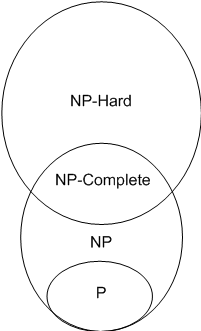
\includegraphics[width=0.3\linewidth]{tex/img/complexity-diagram.png}
	\caption{Venn diagram for the complexity classes if $\mathcal{P} \neq
			\mathcal{NP} $ \cite{article}}%
	\label{fig:tex/img/complexity-diagram}
\end{figure}

\subsection{Optimization Problems and $\mathcal{NPO} $}%
\label{sub:optimization_problems}

Optimization problems are defined from a problem instance $x$, a set of
feasible solutions $S$ and a cost function that takes as input the problem
instance $x$ a feasible solution $s \in S$, denoted as cost$_{O} (x, s) $.
Given a minimization (maximization) problem the optimal solution is defined as
the $s$ minimizing (maximizing) the value of cost$_{O} (x, s)$, and we denote
by opt$_{O} (x) $ this value\cite{Trevisan2004}.

\paragraph{$\mathcal{NPO} $}%
\label{par:_npo_}

is then the set of optimization problems whose cost function
can be computed in polynomial time and for every instance of the problem $x$
and feasible solution for that problem $s \in A$ there is a polynomial $q \; s.t.
	\; s \leq q(|x|)$ (i.e. the size of every solution is bounded by a polynomial
in $x$).

If $\mathcal{P} \neq \mathcal{NP} $ for many optimization problems there is no
algorithm for finding the optimal solution in polynomial time
\cite{Trevisan2004}. This is again a fundamental limitation about what we can
compute which then requires the definition of some alternative approaches, like
the definition of \emph{approximation algorithm}
which are able to be computed in polynomial time
a solution which lies in a given factor from the optimal
one\cite{Vazirani2002}.

\paragraph{Approximation}%
\label{par:r_approximations}

$A$ is an r-approximation algorithm for an $\mathcal{NPO} $ minimization
problem $O$ if, for every instance $x$ of $O$ it holds that
\begin{equation*}
	cost_{O} (x, A(x)) \leq r \cdot opt_{O} (x)
\end{equation*}

\noindent
(or, respectively, cost$_{O} (x, A(x))
	\leq 1/r \cdot $opt$_{O} (x) $ for maximization problems), $A(x)$ being the
optimal solution found by the approximation algorithm \cite{Trevisan2004}.

\subsection{Approximation preserving reductions}%
\label{sub:approximation_preserving_reductions}

Problems approximability varies widely: while for some of them exists
constant factor approximations, for some others even a remotely approximate
solution cannot be found \cite{Ausiello2005} (some examples are listed in
\autoref{tab:inapproximability-examples} ).

% todo: reference to the papers proving each result instead of the hub
\begin{table}
	\centering
	\caption{Examples of known inapproximability results, assuming $\mathcal{P}
			\neq \mathcal{NP} $ \cite{10.1007/3-540-63248-4_10} }
	\label{tab:inapproximability-examples}
	\begin{tabular}{c|p{5cm}|c}
		Problem                                                          & Description                                                   & Inapproximability \\
		\hline
		$ \textsc{MaxClique} $                                           & Biggest complete subgraph                                     & $|V|^{1-
		\epsilon}, \forall \epsilon > 0 $                                                                                                                    \\
		                                                                 &                                                               &                   \\
		$ \textsc{MaximumIndipendentSet} $                               &
		Biggest set of not connected nodes                               & $|V|^{1-
		\epsilon}, \forall \epsilon > 0 $                                                                                                                    \\
		                                                                 &                                                               &                   \\
		$ \textsc{MinCut} $                                              & Partition of nodes in 2 sets $V_1$ and $V_2$ minimizing edges
		between the 2 sets                                               & 1.0624                                                                            \\
		                                                                 &                                                               &                   \\
		$ \textsc{MaximumSetPacking} $                                   & Given a collection of
		finite sets $C$,
		finding the biggest collection $C' \subseteq C$ of disjoint sets & $|C|^{1-
		\epsilon}, \forall \epsilon > 0 $                                                                                                                    \\
	\end{tabular}
\end{table}

\emph{Approximation preserving reductions} are a fundamental notion for proving
a partial order among optimization problems \cite{Ausiello2005}. An
\emph{Approximation preserving reductions} must have
the following properties (when reducing from a problem $A$ to a problem $B$)
\cite{DemaineFall2014}:

\begin{itemize}
	\item any instance $x$ of $A$ should be mapped to an instance $x' = f(x)$
	      of $B$ in polynomial time
	\item any solution $y' \in $ sol$(f(x))$ of $B$ should be associated to a corresponding
	      solution $y = g(x, y') \in $ sol$(x)$ of $A$ in polynomial time
\end{itemize}

So there are 2 efficient (i.e. requiring polynomial time) functions $f$ and $g$
for mapping instances of $A$ to $B$ and solution of $B$ to solutions of $A$,
respectively (\autoref{fig:tex/img/reduction_scheme}).

\begin{figure}
	\centering
	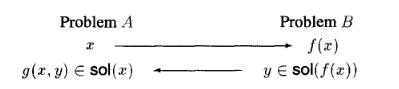
\includegraphics[width=0.6\linewidth]{tex/img/reduction_scheme.png}
	\caption{The reduction scheme \cite{Crescenzi1997ASG}}%
	\label{fig:tex/img/reduction_scheme}
\end{figure}

There are at least 9 different kinds of approximation preserving reductions
\cite{DemaineFall2014}(\autoref{fig:tex/img/approximation_preserving_reductions}) but we will
focus only on one type.

\begin{figure}[b]
	\centering
	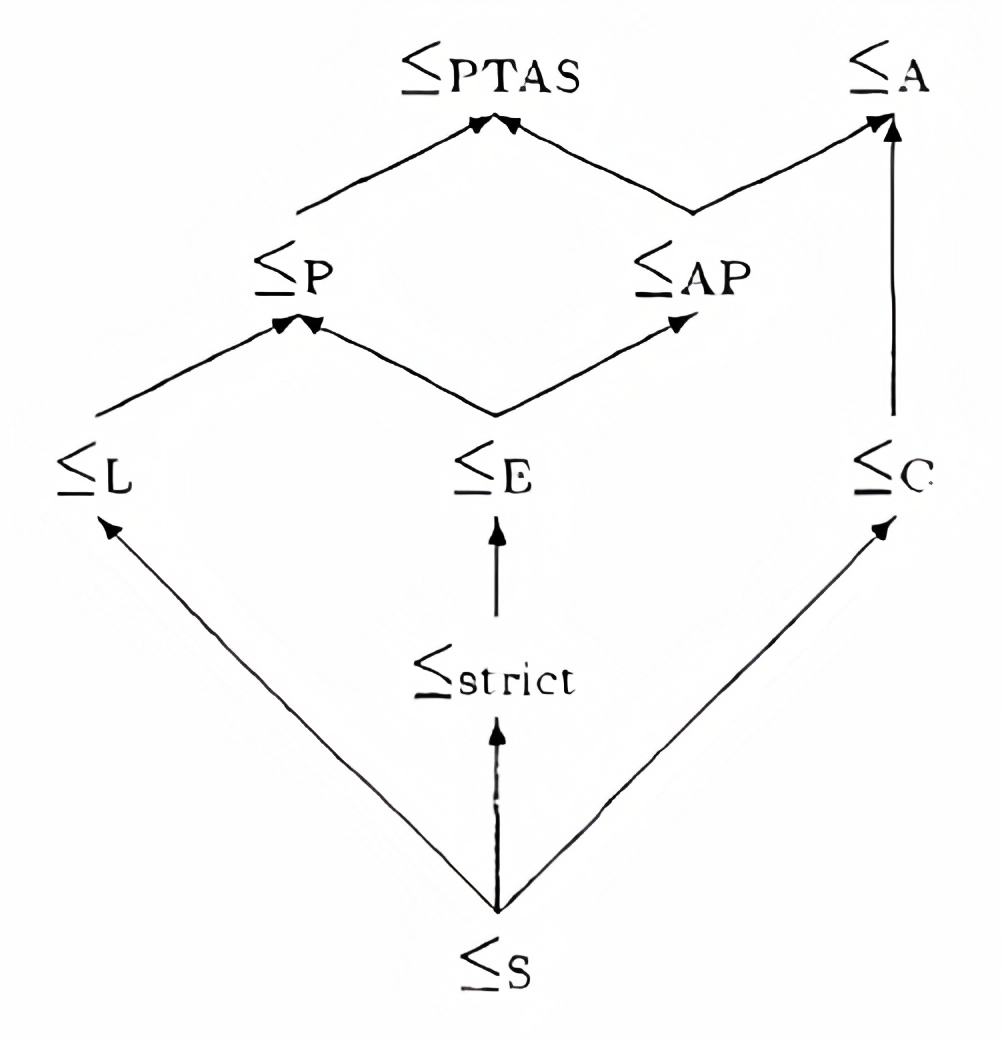
\includegraphics[width=0.4\linewidth]{tex/img/approximation_preserving_reductions.png}
	\caption{Taxonomy of approximation preserving reductions \cite{Crescenzi1997ASG}}%
	\label{fig:tex/img/approximation_preserving_reductions}
\end{figure}

\subsubsection{S reductions}%
\label{sub:strict_reductions}

An $S$ \emph{reduction} from problem $A$ to problem $B$ has the following properties \cite{Crescenzi1997ASG}:
\begin{itemize}
	\item fox any instance $x$ of problem $A$ it holds that opt$_{A} (x) = $ opt$_{B} (f(x))$
	\item for any instance $x$ of $A$ and solution $y'$ of $B$, cost$_{A} (x,
		      g(x, y')) = $ cost$_{B} (f(x), y')$
\end{itemize}

Strict reductions are the strongest type of \emph{approximation preserving
	reductions} and imply all the others \cite{Crescenzi1997ASG}.

\clearpage

\section{Linear and Mixed Integer Programming}%
\label{sec:linear_and_mixed_integer_programming}

\acrlong{LP} is a widely used optimization technique and one of the most
effective; the term refers to problems in which both the constraints and \emph{objective
	function} are linear
\cite{Edgar2001}\cite{Vanderbei2008}\cite{Dantzig1998}\cite{Martin1998}.

\subsection{The structure of a linear programming model}%
\label{sub:the_structure_of_a_linear_programming_model}

In a \acrfull{LP} problem we are given a vector $ \mathbf{c} = (c_1,
	\dots, c_n) $ and we want to maximize (or minimize) a linear function over
the variables $ \mathbf{x} = (x_1, \dots, x_n) $ with the coefficients of the
vector $ \mathbf{c} $, i.e.
\begin{equation*}
	\mathbf{cx} = \sum^{n}_{i=1} c_i x_i
\end{equation*}
(known as the \emph{objective function}) while satisfying some linear
constraints over the variables \cite{Bertsimas1997}\cite{Vanderbei2008}:

\begin{equation*}
	a_1 x_1 + \dots + a_n x_n \begin{Bmatrix} \leq \\ = \\ \geq \end{Bmatrix} b
\end{equation*}

% There is no \emp{a priori} preference regarding how the problem is formulated
% since it is easy to convert an inequality into a equality constraint through
% additional variables ($\omega $ in the example below) called \emph{slack}
% \cite{Vanderbei2008}. For example one in the form
% \begin{equation*}
%     a_1 x_1 + \dots + a_n x_n \leq b
% \end{equation*}
% is equivalent to
% \begin{equation*}
%     a_1 x_1 + \dots + a_n x_n + \omega = b, \quad \omega \geq 0
% \end{equation*}
% and viceversa an equality
% \begin{equation*}
%     a_1 x_1 + \dots + a_n x_n = b
% \end{equation*}
% can be converted into
% \begin{align*}
%     a_1 x_1 + \dots + a_n x_n \leq b \\
%     a_1 x_1 + \dots + a_n x_n \geq b
% \end{align*}
%
In general is possible to formulate any \acrshort{LP} problem as follows (called \emph{standard form}) \cite{Vanderbei2008}

\begin{alignat}{3}
	\label{eq:standard-form}
	\begin{aligned}[t]
		\text{maximize}   &       & \sum_{i=1}^{n} c_{i}x_{i}                                          \\
		\text{subject to} & \quad & \sum_{i=1}^{n} a_{1i}  x_{i} & \leq b_{1} &                        \\
		                  &       & \vdots                                                             \\
		                  &       & \sum_{i=1}^{n} a_{mi}  x_{i} & \leq b_{m} &                        \\
		                  &       & x_{i}                        & \geq 0,    & \quad i & =1 ,\dots, n
	\end{aligned}
\end{alignat}


The $x_i$ are known also as \emph{decision variables}; a choice of $ \mathbf{x}
$ if called \emph{solution} and \emph{feasible solution} if it satisfies the
constraints, \emph{optimum} if it maximizes the \emph{objective function}
\cite{Vanderbei2008}.

\subsection{Solving an LP problem}%
\label{sub:solving_an_lp_problem}

Solving an \acrshort{LP} problem involves a process called the \emph{simplex
	method} which has 2 different phases.

Starting from the \emph{standard form} (\autoref{eq:standard-form})
\emph{slack} variables $x_{n+1}, \dots, $ $x_{n+m} $ are introduced as well as a name
for the \emph{objective} function, allowing to express the problem as follows
\cite{Vanderbei2008}\cite{Edgar2001}

\begin{alignat}{2}
	\label{eq:standard-form}
	 &  & \quad &
	\begin{aligned}[t]
		\zeta   & = \sum_{i=1}^{n} c_{i}x_{i}                                       \\
		x_{n+1} & = b_{1} - \sum_{i=1}^{n} a_{1i}  x_{i} &                          \\
		\vdots                                                                      \\
		x_{n+m} & = b_{m} - \sum_{i=1}^{n} a_{mi}  x_{i} &                          \\
		x_{i}   & \geq 0,                                & \quad i & =1 ,\dots, n+m
	\end{aligned}
\end{alignat}

The first phase involves finding a feasible solution for the problem. More
specifically, we look for $m$ variables, called \emph{basic variables}, whose
value we choose in order to satisfy the $m$ equality constraints (while the
remaining variables, the \emph{nonbasic} ones, are set to 0); if no such
feasible solution exists then the problem is \emph{unfeasible}. Let $\mathcal{B}
$ be the set of \emph{basic variables} and $\mathcal{N} $ the set of
\emph{nonbasic variables} \cite{Vanderbei2008}\cite{Bertsimas1997}. Then the
problem can be reformulated as follows

\begin{alignat}{2}
	\label{eq:standard-form-simplex-new}
	 &  & \quad &
	\begin{aligned}[t]
		\zeta & = \bar{\zeta} + \sum_{j \in \mathcal{N} }^{n} c_{j}x_{j}                                      \\
		x_{i} & = \bar{b}_{i} - \sum_{j \in \mathcal{N} }^{n} \bar{a}_{ij}
		x_{j} & i                                                          & \in \mathcal{B}                  \\
		x_{i} & \geq 0,                                                    & \quad i         & =1 ,\dots, n+m
	\end{aligned}
\end{alignat}

The second phase of the \emph{simplex method} aims at improving the current
solution: if $c_{j} \geq 0, \; \forall j \in \mathcal{N} $ then the value of the
objective function cannot be increased and we found an optimum. If, instead, there is at least a $c_{j}
	> 0$ then we can increase the value of $\zeta$ by increasing $x_{j} $; now
there are 2 different cases \cite{Vanderbei2008}
\begin{itemize}
	\item as $x_{j} $ increases there is at least a variable $\tilde{x}_{j} $
	      whose value needs to decrease to satisfy equality constraints. The first
	      of these variables $\tilde{x}_{j} $ reaching to $0$ moves from
	      $\mathcal{B} $ to $\mathcal{N} $, while
	      $x_{j} $ moves from $\mathcal{N} $ to $\mathcal{B} $. The problem is reformulated again as in
	      \autoref{eq:standard-form-simplex-new} and the process is repeated
	      \cite{Vanderbei2008}.
	\item if no such $\tilde{x}_{j} $ variable exists then the value of $x_{j}
	      $ can be increased indefinitely and the problem is said to be
	      \emph{unbounded}, i.e. it can achieve any arbitrarily large value.
\end{itemize}

The process is illustrated in \autoref{fig:tex/img/simplex}.

\begin{figure}
	\centering
	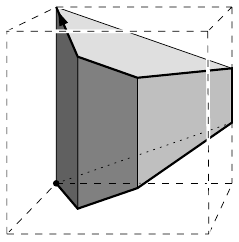
\includegraphics[width=0.4\linewidth]{tex/img/simplex.png}
	\caption{An example of the progress of the \emph{simplex method}: the
		process moves along the vertices of the polygon defined by the
		contraints while improving the value of the solution \cite{BerndGaertner2006}}%
	\label{fig:tex/img/simplex}
\end{figure}

\subsection{Mixed Integer Programming}%
\label{sub:mixed_integer_programming}

Many problems involve not only continous variables but also variable that take binary or
integer values: these are known as \acrfull{MIP} problems. Furthermore, some of
these problems are linear in the constraints and objective function and are
known as \acrfull{MILP} problems
\cite{Edgar2001}\cite{Wolsey1998}.

A generic \acrshort{MILP} can be expressed as \cite{Conforti2016}

\begin{alignat}{3}
	\label{eq:standard-form-milp}
	\begin{aligned}[t]
		\text{maximize}   &                                     & \sum_{i=1}^{n_{1} } c_{i}x_{i} +
		\sum_{i=1}^{n_{2} } h_{i}y_{i}                                                                                                                               \\
		\text{subject to} & \quad                               & \sum_{i=1}^{n_{1} } a_{1i}  x_{i} + \sum_{i=1}^{n_{2} } g_{1i}  y_{i} & \leq b_{1}       &         \\
		                  &                                     & \vdots                                                                                             \\
		                  &                                     & \sum_{i=1}^{n_{1} } a_{mi}  x_{i} + \sum_{i=1}^{n_{2} } g_{1i}  y_{i} & \leq b_{m}       &         \\
		% &       & \sum_{i=1}^{n} a_{mi}  x_{i}                                          & \leq b_{m} &                        \\
		                  &                                     & x_{i}
		                  & \geq 0,                             & \quad i                                                               & =1 ,\dots, n_{1}           \\
		                  &                                     & y_{i}                                                                 & \geq 0,          & \quad i
		                  & =1 ,\dots, n_{2} \; \text{integral}
	\end{aligned}
\end{alignat}

For convenience we will refer to \acrshort{MILP} problems as \acrshort{MIP} in
the rest of the document.

The \emph{relaxation} of a \acrshort{MIP} problem is defined as the same
problem where the integrality constraints have been removed \cite{Edgar2001}.

Solving a \acrshort{MILP} is a difficult task in general, differently from the
\acrshort{LP} problems. It has been shown also that \acrshort{MIP} is
$\mathcal{NP}$-\textbf{Hard}
\cite{Kannan1978}\cite{Liberti2019}\cite{Schrijver1998}. This is why the \emph{relaxation} is often considered
to get an approximation of the exact solution and it is much easier
\cite{Conforti2016}.

\subsection{Solving a MIP}%
\label{sub:solving_a_mip}

One approach that has been proven successfull for solving \acrshort{MIP} is th
e Branch-and-Bound, which is guaranteed to find an optimal solution
\cite{Conforti2016}\cite{Edgar2001}.

Given a problem $P$ the process starts by solving the \emph{relaxation} of $P$
and finding its optimal solution $(\tilde{x}, \tilde{y})$.
Let $S$ and  $\tilde{S}$ be the set of feasible solutions
for the original problem $A$ and its relaxation, respectively. By definition
we have that $S \subseteq \tilde{S} $.
Therefore \cite{Edgar2001}
\begin{itemize}
	\item If the relaxation problem is not feasible so will also the original
	      problem
	\item If $\tilde{y}$ has only integer values then we found the optimal
	      solution for the original problem $A$
\end{itemize}

If, instead, $\tilde{y}$ contains some fractional values, we start by
initialing the value of the best solution so far, $\zeta$, with $-\infty$.
Then we choose one of the fractional variables that are required to be integral
in the original problem $A$, say $y_j$ with value $f$, and create $2$
subproblems, respectively adding the constraint $y_{j} \leq \lfloor f \rfloor$
and $y_{j} \geq \lceil f \rceil$. This step is called \emph{branching}. We now
consider the solution of each subproblem $(x_j, y_j)$ with value of the
objective function $z_{j} $ \cite{Edgar2001}\cite{Conforti2016}.

\begin{itemize}
	\item If either of the subproblems is not feasible or its value $z_{j} $ is
	      lower then the best one found so far then it does not to be
	      considered further. This is called \emph{pruning}.
	\item otherwise if $y_{j} $ are all integer values then $\zeta = z_{j} $
	\item otherwise we subdivide again in $2$ subproblems as done above.
\end{itemize}

When there are no remaining subproblems to consider the Branch-and-Bound method
terminates \cite{Edgar2001}.

\section{Related work}%
\label{sec:related_work}
